\documentclass[10pt]{article}
\usepackage[a4paper,margin=2.2cm]{geometry}
\usepackage{amsmath,amssymb}
\usepackage{graphicx}
\usepackage{booktabs}
\usepackage[font=small,labelfont=bf]{caption}
\usepackage[colorlinks,linkcolor=blue,urlcolor=blue,citecolor=blue]{hyperref}
\graphicspath{{../../figures/}}

\title{\textbf{Physics-Informed Neural Networks for 1D Heat Diffusion:\\Forward Solution and Diffusivity Identification from Noisy Data}}
\author{Quentin Pontalier}
\date{Technical note --- \today}

\begin{document}
\maketitle

\begin{abstract}
\noindent This note summarizes a personal study of physics-informed neural networks (PINNs) on the one-dimensional heat equation. A compact JAX implementation with hard-constrained initial and boundary conditions and L-BFGS optimization solves the forward problem with a relative $L^2$ error of $6\times10^{-5}$ without any data. The same network recovers the thermal diffusivity from about 25 noisy measurements within a few percent. The main difficulty of the inverse problem is \emph{parameter identifiability}: only a restricted region of the space--time domain carries information about $\alpha$. A two-stage sensitivity-weighted data loss is investigated as a way to exploit this structure. Code: \url{https://github.com/qp-dev-ai/pinn-heat-diffusion_1D}.
\end{abstract}

\section{Problem}
Following the PINN framework~	te{raissi2019}, we consider
\begin{equation}
\partial_t T = \alpha\, \partial_{xx} T, \quad x\in[0,1],\ t\in[0,1.5], \qquad T(x,0)=\sin(\pi x),\quad T(0,t)=T(1,t)=0,
\end{equation}
with exact solution $T(x,t)=\sin(\pi x)\,e^{-\alpha\pi^2 t}$. The exact solution is used only to generate synthetic data and to evaluate errors. In the \emph{forward} problem $\alpha$ is known. In the \emph{inverse} problem $\alpha$ is unknown and must be estimated, together with $T$, from $N_d\approx 25$ measurements $T_i^{\mathrm{obs}} = T(x_i,t_i)+\varepsilon_i$ at random locations. The noise is $\varepsilon_i\sim\mathcal{N}(0,\sigma^2)$ with $\sigma = \eta\,\mathrm{std}(T)$ and $\eta\in\{5,10,20\}\%$. Measurements with $T^{\mathrm{obs}}<0$ lie below the noise floor and are discarded.

\section{Method}
\paragraph{Network and hard constraints.} A fully connected network $\mathcal{N}_\theta(x,t)$ (3 hidden layers of 16 neurons, $\tanh$, Glorot-uniform initialization~\cite{glorot2010}) is embedded in the ansatz
\begin{equation}
T_\theta(x,t) = \sin(\pi x) + t\,x\,(1-x)\,\mathcal{N}_\theta(x,t),
\end{equation}
which satisfies the initial and boundary conditions exactly for any weights~\cite{lagaris1998}. This removes the IC/BC penalty terms and their weighting coefficients.

\paragraph{Loss.} The PDE residual $R=\partial_t T_\theta-\alpha\,\partial_{xx}T_\theta$ is computed by automatic differentiation on $N_f=500$ collocation points drawn by Latin Hypercube Sampling. The loss is
\begin{equation}
\mathcal{L}(\theta,\alpha) = \frac{1}{N_f}\sum_{j=1}^{N_f} R(x_j,t_j)^2 \;+\; \lambda\,\frac{\sum_i w_i\,\big(T_\theta(x_i,t_i)-T_i^{\mathrm{obs}}\big)^2}{\sum_i w_i},
\end{equation}
with $w_i=1$ unless stated otherwise. In the inverse problem, positivity of the diffusivity is enforced by the reparameterization $\alpha=\alpha_{\min}+\beta^2$, where $\beta$ is trained jointly with $\theta$.

\paragraph{Optimization.} All computations use double precision. The loss is minimized with L-BFGS (\texttt{jaxopt}, zoom line search, 3000 iterations) from the initial weights, with no Adam warm-up. The collocation points are kept fixed during the optimization.

\section{Forward problem}
With $\alpha=0.18$ known and no data, the PINN reaches a physics loss of $1.4\times10^{-7}$ and a relative $L^2$ error of $6.3\times10^{-5}$ on a $200\times200$ grid in about 30\,s on a laptop CPU (Fig.~\ref{fig:forward}). The benchmark mainly validates the implementation. For a forward problem like this one, classical solvers remain faster and more accurate.

\begin{figure}[h]
\centering
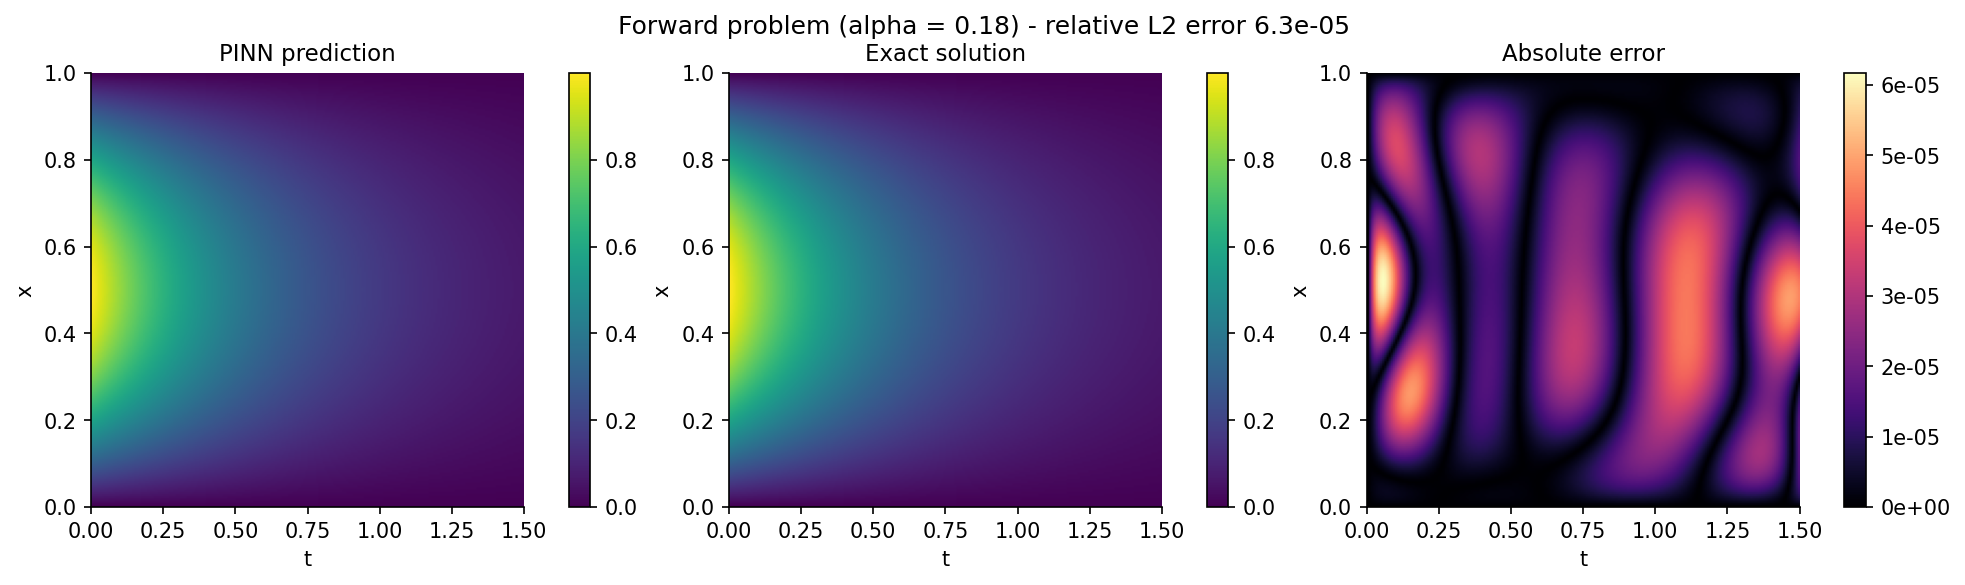
\includegraphics[width=\linewidth]{forward_field.png}
\caption{Forward problem: PINN prediction, exact solution and absolute error.}
\label{fig:forward}
\end{figure}

\section{Inverse problem}
Starting from $\alpha_0=1.0$, the PINN recovers $\hat\alpha=0.1780$ ($1.1\%$ error) from 24 measurements with $10\%$ noise, while reconstructing the full field (Fig.~\ref{fig:inverse}). The estimate first undershoots to $\alpha\approx0.06$ during the early iterations. It then settles once the network has fitted the data.

\begin{figure}[h]
\centering
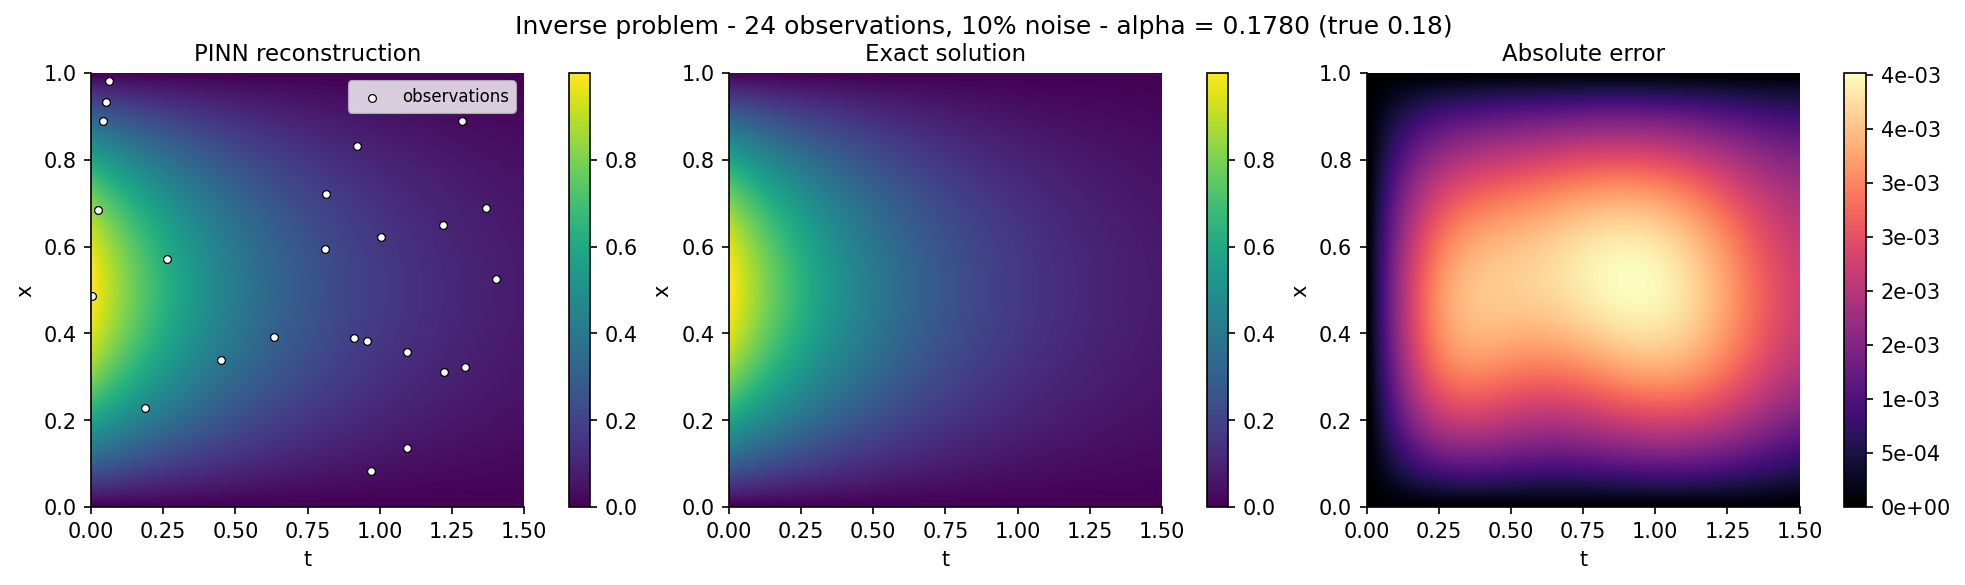
\includegraphics[width=\linewidth]{inverse_field_none.png}
\caption{Inverse problem: reconstructed field with the measurement locations (white dots), exact solution and absolute error.}
\label{fig:inverse}
\end{figure}

\paragraph{Identifiability.} The information that a measurement carries about $\alpha$ is governed by the sensitivity~\cite{beck1977}
\begin{equation}
S_\alpha(x,t)=\frac{\partial T}{\partial\alpha} = -\pi^2\,t\,\sin(\pi x)\,e^{-\alpha\pi^2 t}.
\end{equation}
It vanishes at $t=0$, where the initial profile is independent of $\alpha$, and decays at late times, when the signal falls below the noise. It is maximal at $t^\ast=1/(\alpha\pi^2)$ and $x=1/2$. For independent Gaussian errors, the contribution of a measurement to the Fisher information is proportional to $S_\alpha^2/\sigma^2$. Measurements that are accurate but insensitive therefore constrain $\alpha$ very little. For large $\alpha$ the informative window $t\sim t^\ast$ shrinks, and the temperature field can be fitted with a small error while $\alpha$ is still poorly determined.

\paragraph{Sensitivity-weighted data loss.} To emphasize informative measurements, a two-stage procedure is used. First, an unweighted fit gives $\alpha_1$. Then the network is retrained with
\begin{equation}
w_i=\max\!\Big(\big(|S_\alpha(x_i,t_i;\alpha_1)|/\max_k|S_\alpha(x_k,t_k;\alpha_1)|\big)^{1/2},\; w_{\min}\Big),\qquad w_{\min}=0.05 .
\end{equation}
The square root and the lower bound prevent the loss from concentrating on a few measurements. The weights are applied to the data term only, since the PDE residual must hold throughout the domain. In this benchmark $S_\alpha$ is evaluated analytically; in a real problem it would come from the sensitivity equation or from finite differences of the PINN.

\section{Robustness study}
Each configuration $(\alpha,\eta)$ was solved on three independent random datasets of 25 points, with and without weighting (Fig.~\ref{fig:robust}, Table~\ref{tab:robust}).

\begin{figure}[h]
\centering
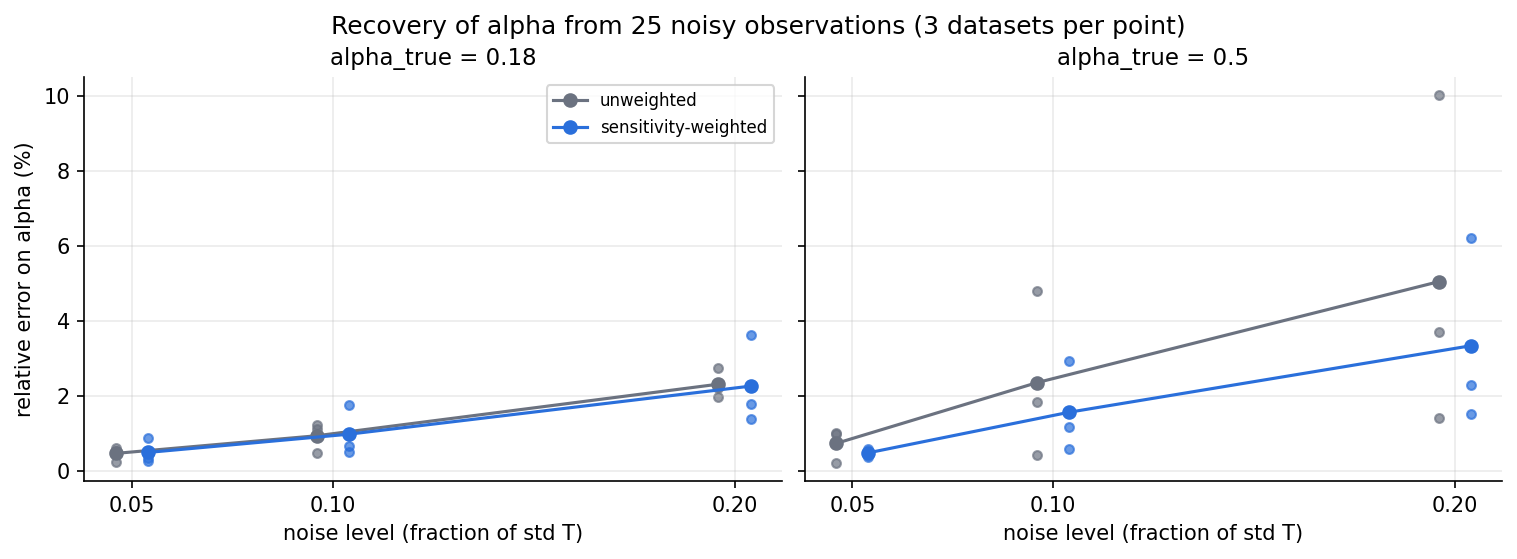
\includegraphics[width=0.9\linewidth]{robustness_study.png}
\caption{Relative error on $\hat\alpha$ against the noise level. Dots are individual datasets; lines are means.}
\label{fig:robust}
\end{figure}

%RESULTS_TABLE

%DISCUSSION

\section{Conclusions and perspectives}
Hard constraints, float64 arithmetic and L-BFGS together give a PINN that is accurate and reproducible on this benchmark. The inverse problem is limited less by the network's ability to approximate the field than by how much information the data carry about the parameter. Every result should therefore be reported over several datasets and seeds. Adaptive loss balancing~	te{wang2021} is a complementary lever that was not used here. Next steps are:
\begin{itemize}
\item estimating the sensitivity without the analytical solution;
\item weak-form (Galerkin) residual constraints;
\item extension to nonlinear diffusion, 2D geometries and experimental data.
\end{itemize}

\begin{thebibliography}{9}\small
\bibitem{raissi2019} M.~Raissi, P.~Perdikaris, G.~E.~Karniadakis, Physics-informed neural networks: A deep learning framework for solving forward and inverse problems involving nonlinear partial differential equations, \emph{J. Comput. Phys.} 378 (2019) 686--707.
\bibitem{glorot2010} X.~Glorot, Y.~Bengio, Understanding the difficulty of training deep feedforward neural networks, \emph{AISTATS} (2010) 249--256.
\bibitem{lagaris1998} I.~E.~Lagaris, A.~Likas, D.~I.~Fotiadis, Artificial neural networks for solving ordinary and partial differential equations, \emph{IEEE Trans. Neural Netw.} 9 (1998) 987--1000.
\bibitem{beck1977} J.~V.~Beck, K.~J.~Arnold, \emph{Parameter Estimation in Engineering and Science}, Wiley (1977).
\bibitem{wang2021} S.~Wang, Y.~Teng, P.~Perdikaris, Understanding and mitigating gradient flow pathologies in physics-informed neural networks, \emph{SIAM J. Sci. Comput.} 43 (2021) A3055--A3081.
\end{thebibliography}

\end{document}
